%%%%%%%%%%%%%%%%%%%%%%%%%%%%%%%%%%%%%%%%%%%%%%%%%%%%%%%%%%%%%%%%%%%%%%%%%%%%%%%%
%2345678901234567890123456789012345678901234567890123456789012345678901234567890
%        1         2         3         4         5         6         7         8

\documentclass[letterpaper, 10 pt, conference]{ieeeconf}  % Comment this line out if you need a4paper

%\documentclass[a4paper, 10pt, conference]{ieeeconf}      % Use this line for a4 paper

\IEEEoverridecommandlockouts                              % This command is only needed if 
                                                          % you want to use the \thanks command

\overrideIEEEmargins                                      % Needed to meet printer requirements.

%In case you encounter the following error:
%Error 1010 The PDF file may be corrupt (unable to open PDF file) OR
%Error 1000 An error occurred while parsing a contents stream. Unable to analyze the PDF file.
%This is a known problem with pdfLaTeX conversion filter. The file cannot be opened with acrobat reader
%Please use one of the alternatives below to circumvent this error by uncommenting one or the other
%\pdfobjcompresslevel=0
%\pdfminorversion=4

% See the \addtolength command later in the file to balance the column lengths
% on the last page of the document

% The following packages can be found on http:\\www.ctan.org
\usepackage{graphics} % for pdf, bitmapped graphics files
\usepackage{epsfig} % for postscript graphics files
\usepackage{mathptmx} % assumes new font selection scheme installed
\usepackage{times} % assumes new font selection scheme installed
\usepackage{amsmath} % assumes amsmath package installed
\usepackage{amssymb}  % assumes amsmath package installed
\usepackage{comment}

\title{\LARGE \bf
Modeling and Simulation of a Three-link Biped 
}


\author{Maxwell Hasenauer, Jarrod Homer, Shreyansh Pitroda, and Dylan Powers % <-this % stops a space
}

\begin{document}



\maketitle
\thispagestyle{empty}
\pagestyle{empty}


%%%%%%%%%%%%%%%%%%%%%%%%%%%%%%%%%%%%%%%%%%%%%%%%%%%%%%%%%%%%%%%%%%%%%%%%%%%%%%%%
\begin{abstract}

This paper presents the modeling and control three-link biped through the method of hybrid zero dynamics (HZD). For modeling and obtaining full dynamical equations, the biped was assumed to have one foot in contact with the ground surface at all times, there is no slippage, and impact with the ground is instantaneous. The full dynamics were then partitioned to obtain zero dynamic equations and gait optimization was performed using Bezier polynomials. Lastly, with the zero dynamics model and an optimized gait, a PD controller was used to drive the system to the zero dynamics manifold, and the results were verified through simulation. 

\end{abstract}


%%%%%%%%%%%%%%%%%%%%%%%%%%%%%%%%%%%%%%%%%%%%%%%%%%%%%%%%%%%%%%%%%%%%%%%%%%%%%%%%
\section{INTRODUCTION}

Locomotion across complicated terrains is a challenging problem that the modern field of robotics is actively solving. Traditionally, the majority of locomotion over land is performed by wheeled vehicles, with cars being the most prevalent. Although, traditional wheeled vehicles inherently have limitations, one-way to break through such limitations is with legged locomotion. 

\indent In nature, terrestrial locomotion is a majority legged locomotion. Legged creatures are able to navigate the most treacherous terrain, and often can go places that a traditional, wheeled vehicle cannot. By studying various creatures, including humans, significant progress has been made in the field of legged locomotion. 

\indent This project dives into the simplified, three-link biped that is model in the sagittal plane of locomotion. The model consists of a stance led, swing leg, and a torso. It is assumed that the model always has one foot in contact with the ground, there is a no slip condition, and impacts are instantaneous. The generalized coordinates of the biped is shown in Figure \ref{model}.

%%%%

\section{Euler-lagrange formalism}
This section outlines the dynamic formulation of the robot which is used for numerical simulation.
%
\begin{figure}
    \centering
    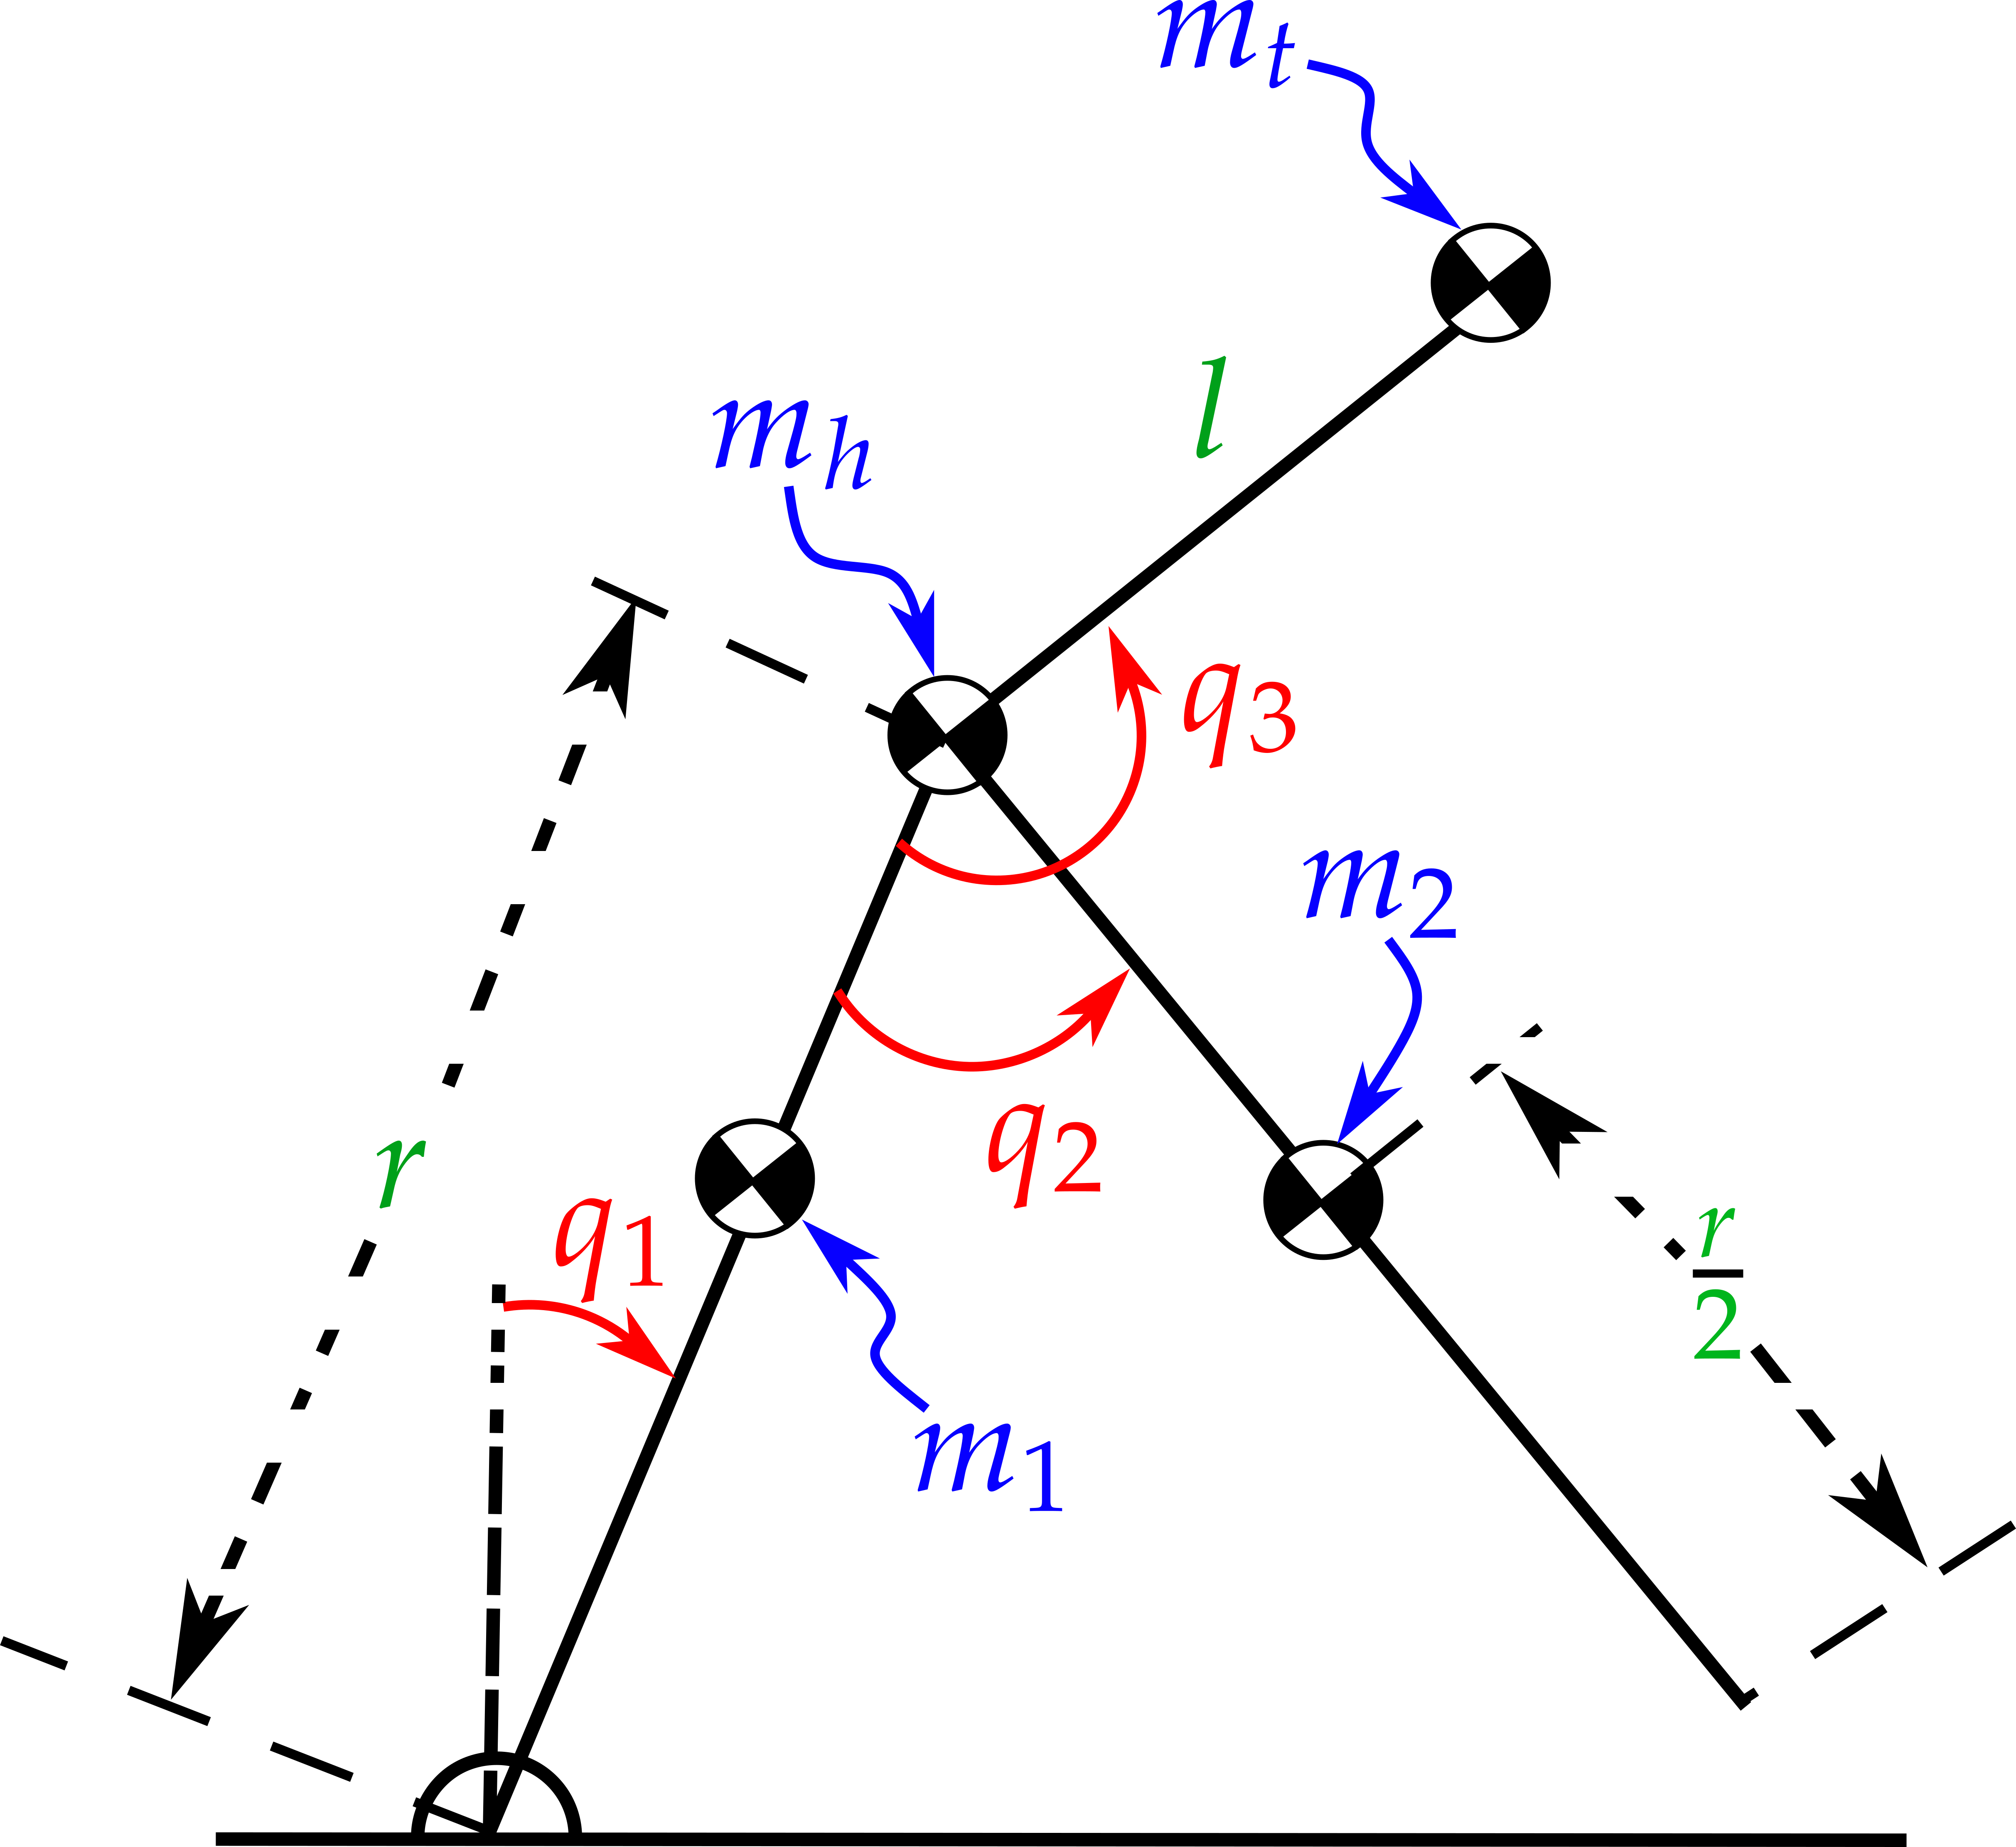
\includegraphics[width=1\linewidth]{Images/Legged_robots_course.png}
    \caption{3 link biped model}
    \label{model}
\end{figure}
%
\subsection{Forward Kinematics}
 Planar biped model consisting of a 3-link pendulum will be used, with relative angles measured counterclockwise as $q_1$, $q_2$, $q_3$ as seen in Figure \ref{model}. Underactuation is located at the point of contact with the ground, at angle $q_1$. 
 
Given that each link as a mass $m_{i}$ and length for stance and swing leg is defined by $r$. Length of torso is $l$ and value for this terms could be found in table [\ref{model params}]

\begin{figure}
\centering
      \begin{tabular}{c c c}\hline
      \bf{Parameter(s)} & \bf{Value} & \bf{description}\\ \hline 
      $m_1$ & $5$ kg & Mass of swing leg \\ \hline
      $m_2$ & $5$ kg & Mass of stance leg \\ \hline
      $m_h$ & $15$ kg & Mass of hip \\ \hline
      $m_t$ & $10$ kg & Mass of torse \\ \hline
      $l$ & $0.5$ m & length of torso \\ \hline
      $r$ & $1$ m & length of each leg \\ \hline
      \end{tabular}
  \caption{Model Parameters} 
  \label{model params}
\end{figure}

%
\begin{equation}
\begin{aligned}
    \theta_{1} &= \pi/2 + q_{1} \\
    \theta_{2} &= q_{2} + q_{1} - \pi/2 \\
    \theta_{3} &= q_{3} + q_{1} - \pi/2 \\
\end{aligned}
\label{absolute angle}
\end{equation}
%

Knowing the absolute joint orientation for each link, we found the position using law of sine and cosine as shown in Equation \ref{FK}

%
\begin{equation}
\begin{aligned}
    P_{mh} &= R(\theta_{1})*[r,0]^{T} \\
    P_{m1} &= R(\theta_{1})*[\frac{r}{2},0]^{T} \\
    P_{m2} &= P_{mh} + R(\theta_{2})*[\frac{r}{2},0]^{T} \\
    P_{mt} &= P_{mh} + R(\theta_{3})*[l,0]^{T} \\
\end{aligned}
\label{FK}
\end{equation}
%
$R(.)$ denotes the rotation matrix in SO ($2$). Further, COM (\ref{Pcm}) and swing leg (\ref{Pswing}) position is found again using forward kinematics.
%
\begin{equation}
\begin{aligned}
    P_{cm} = \frac{P_{mh}*M_{h} + P_{mt}*M_{mt} + (P_{m1} + P_{m2})*M}{M_{mh} + M_{mt} + 2*M} \\
    \end{aligned}
\label{Pcm}
\end{equation}
%

%
\begin{equation}
\begin{aligned}
    P_{2} = P_{mh} + R(\theta_{2})*[r,0]^{T} \\
\end{aligned}
\label{Pswing}
\end{equation}
%
$M_{mh}$,~$M_{mt}$ and~$M$ is the mass at hip, torso and legs respectively. 
Next, velocity of each mass element is found.
%
\begin{equation}
\begin{aligned}
    v = \mathbb{J}\dot{q} \\
\end{aligned}
\label{Pswing}
\end{equation}
%
here ~$\mathbb{J} = \frac{\partial P}{\partial q}$ is the jacobian matrix which relates the joint velocities to the end-effector velocities.

\subsection{Dynamic Modelling}

To further analyze the system's dynamics, we apply the Euler-Lagrange formalism. The Euler-Lagrange equations are derived from the principle of stationary action and relate the Lagrangian of a system to its equations of motion. In our context, the Lagrangian L is the difference between the system's kinetic energy (T) and potential energy (U), i.e., L = T $-$ U.
%
\begin{equation}
\begin{aligned}
    T &= \tfrac{1}{2}\sum_{i \in \mathcal{F}} \left( v_iM_iv_i^{\top} \right) \\
    U &= \sum_{i \in \mathcal{F}} \left( M_igP_{i} \right)
\end{aligned}
\label{energy}
\end{equation}
%
where $\mathcal{F} = \{H,T,sw,st\}$ represents the relevant frames of reference and mass components (Hip, Torso, Swing leg, Stance leg). From the kinetic energy (T) and potential energy(U). Equation of motion in general form legged robot is shown in ~\ref{eom}. 
%
\begin{equation}
\begin{aligned}
    D(q)\ddot{q} + C(q,\dot{q})\dot{q} + G(q) = B(q)u
\end{aligned}
\label{eom}
\end{equation}
%
We can find mass matrix, Coriolis and gravity terms of equation of motion (\ref{eom}) from the kinetic energy (\ref{energy}) and potential energy (\ref{energy}).
%
\begin{equation}
\begin{aligned}
    D(q) = \frac{\partial}{\partial q}\left( \frac{\partial T}{\partial q}\right) 
\end{aligned}
\label{mass matrix}
\end{equation}
%

%
\begin{equation}
\begin{aligned}
    C_{kj} = \frac{1}{2} \sum_{i=1}^{n} \left( \frac{\partial D_{kj}}{\partial q_i} + \frac{\partial D_{ki}}{\partial q_j} - \frac{\partial D_{ij}}{\partial q_k} \right) \dot{q}_i
\end{aligned}
\label{Coriolis matrix}
\end{equation}
%
%
\begin{equation}
\begin{aligned}
     G(q) = \frac{\partial U(q)}{\partial q}
\end{aligned}
\label{gravity martix}
\end{equation}
%
Further, we have one underactuated joint and two actuated joint. so our input matrix is defined by taking differentiating absolute angles (\ref{absolute angle}) with respect to configuration variables ($q_1$, $q_2$, $q_3$)
%
\begin{equation}
\begin{aligned}
     B = \left(\frac{\partial \Theta_{abs}}{\partial q}\right)^\top
\end{aligned}
\label{input martix}
\end{equation}
%
We can represent the system in the form of non-linear state space equation. state vector is given by $x = [q_1,q_2,q_3,\dot{q}_1,\dot{q}_2,\dot{q}_3]^\top$ 
%
\begin{equation}
\begin{aligned}
    \dot{x} = f(x) + g(x)u 
\end{aligned}
\label{Non-linear eom}
\end{equation}
%
%
\begin{equation}
\begin{aligned}
    f(x) = \begin{bmatrix}
    \dot{q}\\
    D^{-1}\left[C(q,\dot{q})\dot{q} + G(q)\right]
    \end{bmatrix}
\end{aligned}
\label{Non-linear state matrix}
\end{equation}
%
\begin{equation}
\begin{aligned}
    g(x) = \begin{bmatrix}
    0\\
    D^{-1}B(q)
    \end{bmatrix}
\end{aligned}
\label{Non-linear input matrix}
\end{equation}
%

\subsection{Unpinned Model}
In the previous section, we assumed that the stance leg is pinned to the ground. This is not ideal as the leg will be fixed to the ground during stance phase and then swing leg will impact ground. So, we need to unpin our model, and we can unpin our model by extending our generalized coordinates.
For the unpinned model, we augment the set of generalized coordinates q with the position of the base frame $\left(H\right)$, $p_e = \left(p^h_e, p^v_e\right)$. Therefore, the new generalized coordinates become $q_e = \left(q, p_e\right)$.\newline

Now, that we obtained our extended generalized coordinates $\left(q_{e}\right)$,we performed the same steps shown in forward kinematics and dynamic modelling to obtain equation of motion for extended system (\ref{extended eom}). 
%
\begin{equation}
\begin{aligned}
    D_e(q_e)\ddot{q_e} + C_e(q_e,\dot{q_e})\dot{q_e} + G(q_e) = B_e(q_e)u
\end{aligned}
\label{extended eom}
\end{equation}
%

\vspace{0.05cm}

\section{Reduced Order Modeling}
This section presents the process of obtaining the reduced order model for the three-link model through partitioning the full-dynamics equations.

\subsection{Full-Dynamics Partitioning}

The dynamic model given by Equation \ref{eom}, was partitioned in the following way:

\begin{equation}
    \scalebox{0.85}{
        $\left[\begin{array}{lll}
            d_{11} & d_{12} & d_{13} \\
            d_{21} & d_{22} & d_{23} \\
            d_{31} & d_{32} & d_{33}
        \end{array}\right]+\left[\begin{array}{l}
            \ddot{q}_1 \\
            \ddot{q}_2 \\
            \ddot{q}_3
        \end{array}\right]+\left[\begin{array}{l}
            H_1 \\
            H_2 \\
            H_3
        \end{array}\right]=\left[\begin{array}{c}
            0 \\
            B_1\left(q_b\right) \\
            B_2\left(q_b\right)
        \end{array}\right] u$
    }
\end{equation}

where

\begin{equation}
q_1=q_N \quad q_b=\left[\begin{array}{ll}
q_2 & q_3
\end{array}\right]^{\top}
\end{equation}

\begin{equation}
\Omega_1=H_1 \quad \Omega_2=\left[\begin{array}{ll}
H_2 & H_3
\end{array}\right]^{\top}
\end{equation}

\begin{equation}
D_{11}=d_{11} \quad D_{12}=\left[\begin{array}{ll}
d_{12} & d_{13}
\end{array}\right]^{\top}
\end{equation}

as shown in

\begin{equation}
\left[\begin{array}{ll}
D_{11} & D_{12} \\
D_{21} & D_{22}
\end{array}\right]\left[\begin{array}{l}
\ddot{q}_N \\
\ddot{q}_b
\end{array}\right]+\left[\begin{array}{c}
\Omega_1 \\
\Omega_2
\end{array}\right]=\left[\begin{array}{c}
0 \\
B\left(q_b\right)
\end{array}\right] u
\end{equation}

\vspace{0.05cm}

\begin{comment}
%K_Mh
\begin{equation}
\begin{aligned}
    K_{Mh} = \frac{1}{2} \cdot M_{h} \cdot (\mathbf{v}_{Mh})^\top (\mathbf{v}_{Mh})
\end{aligned}
\label{K of Hip}
\end{equation}

%K_Mt
\begin{equation}
\begin{aligned}
    K_{Mt} = \frac{1}{2} \cdot M_{t} \cdot (\mathbf{v}_{Mt})^\top (\mathbf{v}_{Mt})
\end{aligned}
\label{K of torso}
\end{equation}

%K_m1
\begin{equation}
\begin{aligned}
    K_{m1} = \frac{1}{2} \cdot M \cdot (\mathbf{v}_{m1})^\top (\mathbf{v}_{m1})
\end{aligned}
\label{K of mass1}
\end{equation}


%K_m2
\begin{equation}
\begin{aligned}
    K_{m2} = \frac{1}{2} \cdot M \cdot (\mathbf{v}_{m2})^\top (\mathbf{v}_{m2})
\end{aligned}
\label{K of mass2}
\end{equation}

%K
\begin{equation}
\begin{aligned}
    K = K_{M_{h}} + K_{M_{t}} + K_{M_{1}} + K_{M_{2}}
\end{aligned}
\label{Total K}
\end{equation}

%V_Mh
\begin{equation}
\begin{aligned}
    V_{M_{h}} = M_{h}gP_{M_{h}}^v
\end{aligned}
\label{V of hip}
\end{equation}

%V_Mt
\begin{equation}
\begin{aligned}
    V_{M_{t}} = M_{t}gP_{M_{t}}^v
\end{aligned}
\label{V of torso}
\end{equation}

%V_m1
\begin{equation}
\begin{aligned}
    V_{M_{1}} = M_{1}gP_{M_{1}}^v
\end{aligned}
\label{V of M1}
\end{equation}

%V_m2
\begin{equation}
\begin{aligned}
    V_{M_{2}} = M_{2}gP_{M_{2}}^v
\end{aligned}
\label{V of M1}
\end{equation}

%V
\begin{equation}
\begin{aligned}
    V = V_{M_{h}} + V_{M_{t}} + V_{M_{1}} + V_{M_{2}}
\end{aligned}
\label{Total V}
\end{equation}

%D Masss Inetia Matrix


%Coriolois

%Gravit vector

%B

\end{comment}

\subsection{Reduced Order Coordinates}
Using the partitioned dynamics, we can now define our system by our cyclic coordinates separately from the body coordinates, using this separation we can then parameterize them by using the cyclic coordinate. First, we can define a new variable called the gait timing by first isolating the cyclic variable fro the rest of the generalized coordinates, using a row vector denoted as c. 
\begin{equation}
\begin{aligned}
    \theta(q) :&= cq = q_N \\
\end{aligned}
\end{equation}
Then, we can normalize the cyclic variable using the values from the beginning and end of the gait, giving us a timing variable for the gait with $s(q) \in [0,1]$. We then can feed this into a bezier equation to get a curve to represent the values of our body variables.
\begin{equation}
\begin{aligned}
    \ s(q) :&= \frac{\theta(q) - \theta^{+}}{\theta^{-} - \theta^{+}} \\
    \ b_i(s) :&= \sum^{M}_{k=0} \alpha^{i}_{k} \frac{M!}{k!(M-k)!} s^{k} (1-s)^{M-k} \\
\end{aligned}
\end{equation}
These bezier curves for our body coordinates are then collected together into a new matrix denoted $h_d(q)$, representing the values of the body coordinates being defined in relation to the value of the cyclic variable. 
\begin{equation}
\begin{aligned}
    h_d(q) \circ \theta(q) :&=
    \begin{bmatrix}
    b_1\circ s(q)\\
    b_2\circ s(q)\\
    \vdots \\
    b_{N-1}\circ s(q)
\end{bmatrix}
\end{aligned}
\end{equation}
Giving us the ability to define our system, instead of the full state space model $x$ $\in$ $\mathbb{R}^{2N}$, our new reduced state space model $z$ $\in$ $\mathbb{R}^2$, where $z:= [q_1,~ \dot{q_1}]$.
\section{Zero Dynamics}
We can use the reduced order model to simplify our system, and impose a series of virtual holonomic constraints using an output equation to limit the system to the 2 dimensional embedded sub-manifold within our state space system defined in set notation
\begin{equation}
\begin{aligned}
    Z := \{x \in \mathbb{R}^{2N} ~|~ y(x) = 0,~ \dot{y}(x) = 0\}
\end{aligned}
\end{equation}
We use the partitioned dynamics to define the relationship from our input, $u$, to our output equation $y$ by taking the relative derivative of our output function until we find the input in the derivative. Using this we can design our input to negate the dynamics of our system, and then also force the system into the Zero Dynamics manifold to enforce stability into the system.


\vspace{0.05cm}

\section{optimization}
After completing the zero dynamics modelling. we use matlab's fmincon optimizer to simulate our zero dynamics model. The optimization parameters used are shown below.

\begin{equation}
    \begin{aligned}
        Z^{-} = \begin{bmatrix}
             -0.349066, -1
        \end{bmatrix}
    \end{aligned}
\label{Z_minus}
\end{equation}

\begin{equation}
    \begin{aligned}
        alpha = \begin{bmatrix}
             0.35, 0.5, 0.698132
        \end{bmatrix}
    \end{aligned}
\label{Bezier_alpha}
\end{equation}

\begin{equation}
    \begin{aligned}
        gamma = \begin{bmatrix}
             2.9, 3.0, 3.0
        \end{bmatrix}
    \end{aligned}
\label{Bezier_gamma}
\end{equation}

After the optimization was complete, the following values were obtained and used for simulating the gait. 

\begin{equation}
    \scalebox{0.75}{$
    \begin{aligned}
        f = \begin{bmatrix}
             -0.2991, -1.0383, 0.3018, 0.4633, 0.6509, 3.0918, 3.0498, 2.9500
        \end{bmatrix}
    \end{aligned}
    $}
\label{f_values}
\end{equation}

%
\begin{figure}
    \centering
    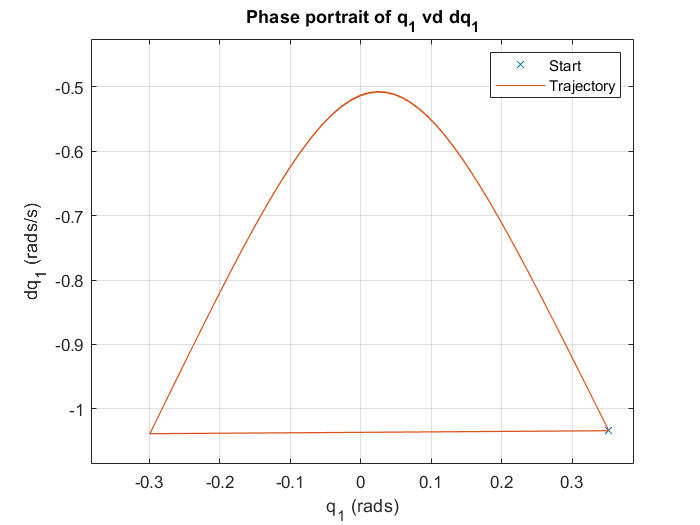
\includegraphics[width=1\linewidth]{Images/Optimization Phase Diagram.png}
    \caption{Phase portrait of q1 and dq1}
    \label{Phase}
\end{figure}
%



\section{Non-linear Controller design}
The common approach used to design controllers for nonlinear systems is feedback linearization. In this study, we will use output feedback linearization to drive our nonlinear system towards the predefined embedded zero dynamics submanifold. We can shape the output of our non linear dynamics (\ref{Non-linear eom}) to perfrom reference tracking.
%
\begin{equation}
\begin{aligned}
    y = h(q) - h_{d}(q) 
\end{aligned}
\label{output function}
\end{equation}
%
here $h(q)$ is the current state of the controlled variable$\left(q_2,q_3 \right)$ of the system. $h_d(q)$ denotes the desired states of these variables defined by the zero dynamics manifold. The objective of the feedback linearization is to minimize the error or in simplier terms drive output function (\ref{output function}) to zero. To achieve this zero dynamic, we employ a PD controller. 
%
\begin{equation}
\begin{aligned}
    v = (K_p)y + (K_d)\dot{y}
\end{aligned}
\label{v}
\end{equation}
%
where, $K_p = diag([10000,2000])$ and $K_d = diag([60,60])$. To find this control input we need to first differentiate our output function (\ref{output function}) until the input to our non-linear dynamics(\ref{Non-linear eom}) shows up. 









%
\begin{equation}
\begin{aligned}
    \dot{y} = \frac{\partial h}{\partial x}\left( f(x) + g(x)u\right)
\end{aligned}
\label{output function}
\end{equation}
%
%
\begin{equation}
\begin{aligned}
    \frac{\partial h}{\partial x} = \begin{bmatrix} 
            -\frac{\partial q_2}{\partial s} & 1 & 0 & 0 & 0 & 0 \\
            -\frac{\partial q_3}{\partial s} & 0 & 1 & 0 & 0 & 0 \\
            \end{bmatrix}
\end{aligned}
\label{derivative of output}
\end{equation}





further, $L_{f}h = \frac{\partial h}{\partial x}\left( f(x)\right)$ is the lie derivative of function $h$ along vector field $f(x)$ and $L_{g}h = \frac{\partial h}{\partial x}\left(g(x)u\right)$ is the lie derivative along vector field $g(x)$. For our system, the input $u$ shows up after taking the second derivative so our for
%
\begin{equation}
\begin{aligned}
    \ddot{y} = \left(L^2_fh + (L_gL_fh)u\right)
\end{aligned}
\label{output function}
\end{equation}




%
\begin{figure*}
    \centering
    \includegraphics[width=\linewidth]{Images/walking.png}
    \caption{Walking}
    \label{Walking}
\end{figure*}
%


%
\begin{figure}
    \centering
    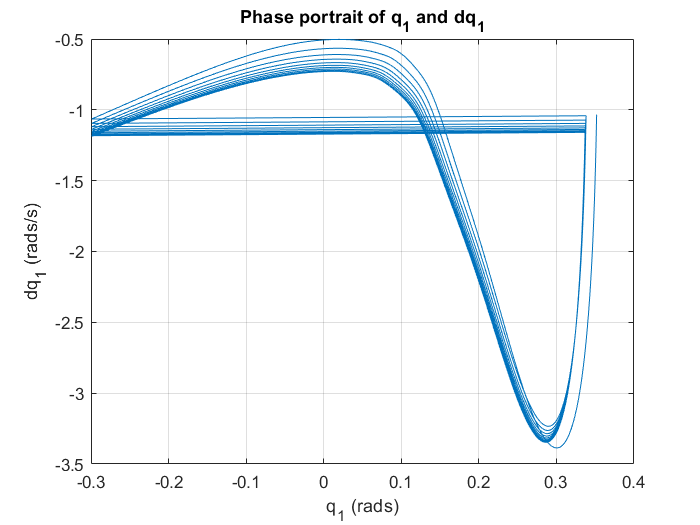
\includegraphics[width=1\linewidth]{Images/Controller Phase Diagram 2.png}
    \caption{Controller q1 Phase Portrait}
    \label{Cont2 Phase q1}
\end{figure}
%


%
\begin{figure}
    \centering
    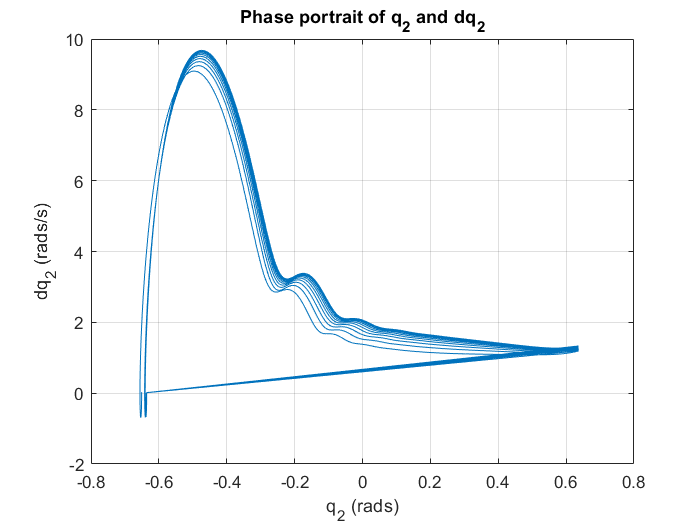
\includegraphics[width=1\linewidth]{Images/Controller Phase Diagram 2 q2.png}
    \caption{Controller q2 Phase Portrait}
    \label{Cont2 Phase q2}
\end{figure}
%

%
\begin{figure}
    \centering
    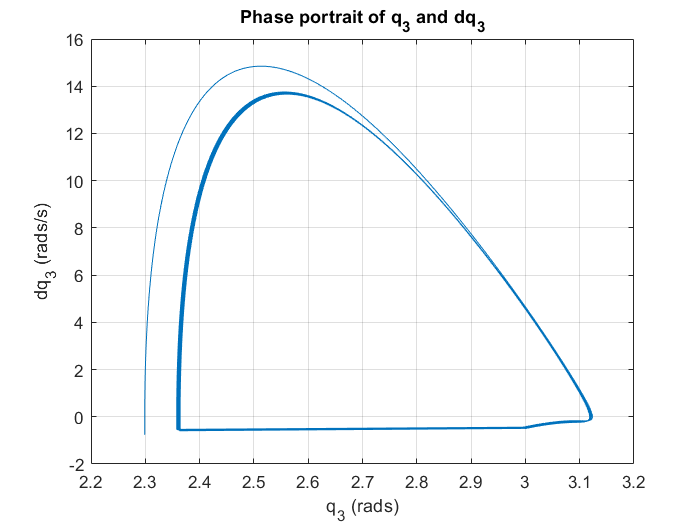
\includegraphics[width=1\linewidth]{Images/Controller Phase Diagram 2 q3.png}
    \caption{Controller q3 Phase Portrait}
    \label{Cont2 Phase q3}
\end{figure}
%



%
\begin{figure}
    \centering
    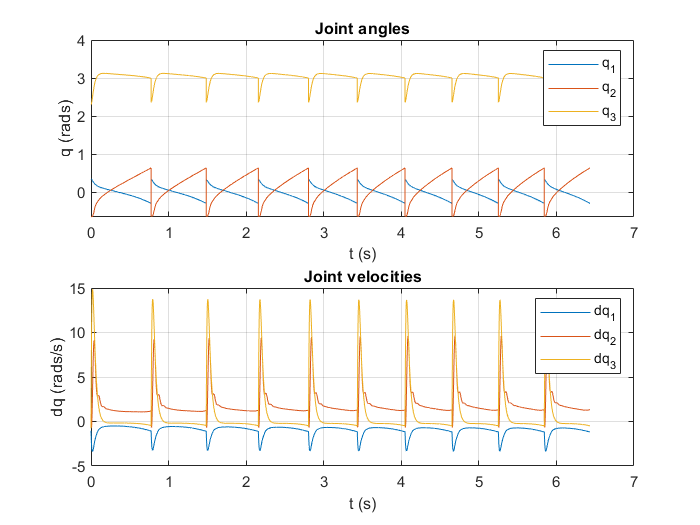
\includegraphics[width=1\linewidth]{Images/Joint Angles and Velocities 2.png}
    \caption{Controller 2 Joint Angles}
    \label{Cont2 Joints}
\end{figure}
%








Now, since we want output$\left(y\right) = 0$ so all the corresponding derivatives will also be zero $\left(\dot{y},\ddot{y}\right)$. Final output which will cancel the dynamics will be







%
\begin{equation}
\begin{aligned}
    u^* = -\left(L_gL_fh\right)^{-1}\left(L^2_fh\right)
\end{aligned}
\label{u*}
\end{equation}
%
%
\begin{equation}
\begin{aligned}
    L^2_fh = \begin{bmatrix} 
            \frac{\partial L_fh}{\partial q} & \frac{\partial h}{\partial q}
            \end{bmatrix}f(x) \\
    L_gL_fh = \begin{bmatrix} 
            \frac{\partial L_fh}{\partial q} & \frac{\partial h}{\partial q}\\
            \end{bmatrix}g(x)    
\end{aligned}
\label{L2f and Lglf}
\end{equation}
%
Finally, the input which will propogate the states in the zero dynamics and which will keep the system bounded to the manifold is give by 
%
\begin{equation}
\begin{aligned}
    u = v + u^*
\end{aligned}
\label{u}
\end{equation}
%
















\section{CONCLUSIONS}
In this work we have looked at kinematics, dynamics gait optimization and controller implementation for a three link walker. This paper has demonstrated the application of HZD in modeling and controlling a simplified three-link biped in the sagittal plane of locomotion. By assuming continuous contact with the ground, no slip conditions, and instantaneous impacts, the full dynamical equations were derived and partitioned to obtain zero dynamic equations. Gait optimization techniques using Bezier polynomials were employed to refine the biped's motion. Subsequently, a proportional-derivative (PD) controller was utilized to guide the system towards the zero dynamics manifold. Through simulation, the effectiveness of the model gait and controller was verified.

\section{FUTURE WORKS}
Our results are promising given the simple 3 link model and naive approach, but there is room for improvement. Using high gains is potentially problematic, so finding a gait that works with lower gains could be more stable and allow the controller to generalize better. The current controller with high gains likely would not work in hardware with the introduction of noise or model inaccuracies. The gait optimization could be improved to make the gait more symmetric. Additionally other types of controllers could be implemented.



\addtolength{\textheight}{-12cm}   % This command serves to balance the column lengths
                                  % on the last page of the document manually. It shortens
                                  % the textheight of the last page by a suitable amount.
                                  % This command does not take effect until the next page
                                  % so it should come on the page before the last. Make
                                  % sure that you do not shorten the textheight too much.

%%%%%%%%%%%%%%%%%%%%%%%%%%%%%%%%%%%%%%%%%%%%%%%%%%%%%%%%%%%%%%%%%%%%%%%%%%%%%%%%



\begin{comment}
    
\begin{thebibliography}{99}


\end{thebibliography}

\end{comment}



\end{document}
